We now define a formalizations of the concepts described in
Section~\ref{sec:problem} and depicted in Figure~\ref{fig:safety-security}. We
base our formalization on first order logic (FOL) with the standard
truth-value semantics. The choice of this logic is required by the 
semantics of the concepts formalized afterwards in this section. 

We consider a first-order language $\follang$ over a
signature $\Sigma_P$ where $P,P',\ldots,P^n$ represent terms, and
$\varphi,\varphi',\ldots,\varphi^n$ represent formulas.
The syntax is defined as follows.
\begin{displaymath}
	\varphi := P~|~\neg\varphi~|~\varphi\wedge\varphi~|~\varphi\vee\varphi~|~\varphi\Rightarrow\varphi'~|~\forall P.~\varphi~|~\exists P.~\varphi
\end{displaymath}
where $\wedge$, $\neg$, $\vee$, and $\Rightarrow$ are connectives representing
conjunction, negation, disjunction, and (material) implication respectively;
while $\forall$ and $\exists$ represent the standard universal and existential
quantifiers (resp.). Finally, the symbol ``$.$'' is just syntactic sugar.  We
consider $\interpretation\subset\Phi\times\{\top,\bot\}$ as the interpretation
function, where $\Phi$ is any collection of sentences in $\follang$ and $\top$
and $\bot$ represent the concepts of ``Tautology/True'' and
``Contradiction/False'' respectively.

Following Figure~\ref{fig:safety-security}, we start by formalizing the outermost term: Causality.

\subsection{Causality Principle}\label{sec:causality}
We formalize the Causality Principle starting from a K modal
logic\autocite{Garson2018modal} (i.e. without restrictions on the causality
relation between worlds). The standard definition of K modal logic is given in
Definition~\ref{def:modallogic} in terms of an interpretation function (which
we named $\sigma$ with a slight abuse of notation) defined in
Definition~\ref{def:modalinterpretation}. 
\begin{definition}{\bf K Modal Logic --}\label{def:modallogic}
A K-frame is a frame $ \kframe=\langle \possibleworlds,\modalrelation \rangle $
	in the K modal logic where $ \modalrelation $ is the binary relation
	(i.e. a set of ordered pairs) between possible worlds
	$\modalrelation\subseteq\possibleworlds\times\possibleworlds$, where
	$\possibleworlds$ represents the possible worlds, and
	$\possibleworlds\neq\emptyset$. An actual world
	$\actualworld\in\possibleworlds$ is assumed. For any proposition $P$,
	an interpretation function $\interpretation(\world,P)$ returns the
	truth value of $P$; e.g. $\interpretation(\world,P)=\top$ means that
	$P$ holds in $\world$. A model is defined as the tuple
	$\kmodel=\langle\possibleworlds,\modalrelation,\interpretation\rangle$.
\end{definition}

\begin{definition}{\bf Causality as K Modal Interpretation Function --}\label{def:modalinterpretation}
	Causality is (recursively) defined as the modal interpretation function $\interpretation$, as follows. 
	\begin{enumerate}[noitemsep]
		\item[$(\interpretation0)$] if $\interpretation(\world,P)=\top$ then $\world\models P$
		\item[$(\interpretation1)$] $\world\models\neg P$ iff $\world\not\models P$
		\item[$(\interpretation2)$] $\world\models P \wedge Q$ iff $\world\models P$ and $\world\models Q$
		\item[$(\interpretation3)$] $\world\models\Box P$ iff for any world $\world'\in\possibleworlds$ if $\world \modalrelation\world'$ then $\world'\models P$
		\item[$(\interpretation4)$] $\world\models\Diamond P$ iff there exists a set of worlds $\World'\subset\possibleworlds$ such that for any $\world'\in\World'$, if $\world\modalrelation\world'$ then $\world'\models P$
		\item[$(\interpretation5)$] $\models P$ iff $\actualworld\models P$
	\end{enumerate}
	where truth is defined as necessary with $\Box$ and possible with $\Diamond$.
\end{definition}

The causality principle has been defined in its generic form. In fact, the
accessibility relation $\modalrelation$ is free from any axiomatic restriction
(e.g. it's not reflexive nor anti-reflexive).  We will focus in
Section~\ref{sec:engineering} (for our tests) on the application of our theory
to CPS system engineering.  More detailed case studies (i.e. \fix{mr}{a CPS as
a smart power-grid}) will be defined in Section~\ref{sec:engineering}, where
the accessibility relation defines in details how the system itself evolves,
due to causal relation (i.e. by restricting the causality principle only to
those cause-effect that defines the system). Therefore, the definition of
$\modalrelation$ will be specialized in a more strict way based on the
application domains and case study.

We note that we have defined the Causality principle without considering it a
\emph{threat source} since we lack the concept of intent and maliciousness.
Similarly, in the next sections we won't discriminate between Nature and
Mankind until we introduce the concepts of maliciousness in
Section~\ref{sec:theory} and then formally define a threat agent in the same
section.

\subsection{Agents: Mankind and Nature}\label{sec:mankind-nature}
\begin{table}[t]
\centering
\setlength{\tabcolsep}{3.5pt}
\renewcommand{\arraystretch}{1}
\scriptsize
\caption{RCC3, RCC5, and RCC8 relations between Regions $X$, $Y$ and $Z$ ~\label{tab:rcc358}~\label{tab:rcc}}
\begin{tabular}{ccclll} 
\rota{\textbf{RCC3}}&\rota{\textbf{RCC5}}&\rota{\textbf{RCC8}}&\textbf{Name} & \textbf{Notation} & \textbf{Definition} \\
\hline
&&&Connects with 			& $\mathit{C}(\mathit{X},\mathit{Y})$ 		& $\mathit{X}\subseteq \mathit{Y}$ \\
&&&Disconnected from		& $\neg \mathit{C}(\mathit{X},\mathit{Y})$		& $\mathit{X}\not\subseteq \mathit{Y}$\\
&&&Part of				& $\mathit{P}(\mathit{X},\mathit{Y})$		& $\forall \mathit{Z} ~\mathit{C}(\mathit{Z},\mathit{X}) \rightarrow \mathit{C}(\mathit{Z},\mathit{Y})$\\
&&&Overlaps			& $\mathit{O}(\mathit{X},\mathit{Y})$		& $\exists \mathit{Z} ~\mathit{P}(\mathit{Z},\mathit{X})\wedge \mathit{P}(\mathit{Z},\mathit{Y})$\\
\Tdot&&&  \textbf{Overlaps Not Equal} 	& $\mathit{ONE}(\mathit{X},\mathit{Y})$		& $\mathit{O}(\mathit{X},\mathit{Y}) \land \neg \mathit{EQ}(\mathit{X},\mathit{Y})$ \\
\Tdot&\Tdot&\Tdot& \textbf{Equal to} 		& $\mathit{EQ}(\mathit{X},\mathit{Y})$  		& $\mathit{P}(\mathit{X},\mathit{Y}) \wedge \mathit{P}(\mathit{Y},\mathit{X})$\\
\Tdot&\Tdot&\Tdot& \textbf{DiscRete from} 		& $\mathit{DR}(\mathit{X},\mathit{Y})$		& $\neg \mathit{O}(\mathit{X},\mathit{Y})$\\
&\Tdot&\Tdot&\textbf{Partial-Overlap}	& $\mathit{PO}(\mathit{X},\mathit{Y})$ 		& $\mathit{O}(\mathit{X},\mathit{Y})\wedge \neg \mathit{P}(\mathit{X},\mathit{Y}) \wedge \neg \mathit{P}(\mathit{Y},\mathit{X})$\\ 
&\Tdot&&\textbf{Proper-Part-of} 	& $\mathit{PP}(\mathit{X},\mathit{Y})$ 		& $\mathit{P}(\mathit{X},\mathit{Y})\wedge \neg \mathit{P}(\mathit{Y},\mathit{X})$\\ 
	&\Tdot&&\textbf{Proper-Part-of-\textit{\textbf{i}}nverse} & $\mathit{PPi}(\mathit{X},\mathit{Y})$ 		& $\mathit{P}(\mathit{Y},\mathit{X}) \wedge \neg \mathit{P}(\mathit{X},\mathit{Y})$\\
&&\Tdot&\textbf{Externally Connected} 	& $\mathit{EC}(\mathit{X},\mathit{Y})$ 		& $\mathit{C}(\mathit{X},\mathit{Y}) \wedge \neg\mathit{O}(\mathit{X},\mathit{Y})$\\ 
&&\Tdot&\textbf{Tangential PP} 	& $\mathit{TPP}(\mathit{X},\mathit{Y})$ 		& $\mathit{PP}(\mathit{X},\mathit{Y})\wedge\exists\mathit{Z}~[\mathit{EC}(\mathit{Z},\mathit{X}),\mathit{EC}(\mathit{Z},\mathit{Y})]$\\ 
&&\Tdot&\textbf{Tangential PPi} 	& $\mathit{TPPi}(\mathit{X},\mathit{Y})$ 		& $\mathit{TPP}(\mathit{Y},\mathit{X})$\\ 
&&\Tdot&\textbf{Non-Tangential PP} 	& $\mathit{NTPP}(\mathit{X},\mathit{Y})$ 		& $\mathit{PP}(\mathit{X},\mathit{Y})\wedge\neg\exists\mathit{Z}~[\mathit{EC}(\mathit{Z},\mathit{X}),\mathit{EC}(\mathit{Z},\mathit{Y})]$\\ 
&&\Tdot&\textbf{Non-Tangential PPi} 	& $\mathit{NTPPi}(\mathit{X},\mathit{Y})$ 		& $\mathit{NTPP}(\mathit{Y},\mathit{X})$\\ 
\end{tabular}
\end{table}

Mankind and Nature are considered as two abstract
agents, both defined as collections (i.e. an abstract type that does not imply a
specific implementation) of their sub-agents (i.e. humans for Mankind and
plants, animals, \&c.  for Nature). Similarly to\autocite{Santaca2016abf}, we
define Mankind and Nature, and any other agent in the reminder of this article,
as a meronomy (an hierarchy of Part-Whole relations) based on a standard
definition of mereology, i.e. based on the definition of Parthood relation
between \emph{Parts}.  However, we consider different types of Part; so, we
extend the mereology to a
mereo-topology\autocite{Smith1996mereotopology,Varzi1994mereotopology,Rachavelpula2017mereotopology},
to increase the number of different types considered and to generalize the
relations between Parts (as in Table~\ref{tab:rcc358}).  For the sake of
readability, we use the term \emph{Region} both to refer to a mereological Part
and to a topological Region.  The choice of mereotopology is also correlated to
the objective of defining a formal ontology, which we use to define the
(formal) semantics of the terms (Parts) in Section~\ref{sec:problem}, and of
the concepts of safety and security (whole). We aim at creating a meronomy
instead of the taxonomies such as the one provided
in\autocite{NIST2020NVD,MITRE2020CVE} or instead of the poorly justified
CVSS\autocite{Mell2007CVSS} scoring system.  

A mereotopology, as defined e.g. in\autocite{Rachavelpula2017mereotopology},
is an ordered mathematical structure where the basic relation between Regions is the
reflexive and symmetric\fixnote{mr}{I guess it must be monotonic as defined in\autocite{Rachavelpula2017mereotopology} but I don't find it consistently in other papers.} 
\emph{Parthood} relation $\subseteq$. 
\begin{definition}{\bf Parthood --}\label{def:parthood}
Given any pair of mereotopological Regions $X$ and $Y$,
	\begin{enumerate}[noitemsep]
		\item Reflexivity: $\forall X.~ (X\subseteq X)$
		\item Symmetry: $\forall X, Y.~ (X\subseteq Y \Rightarrow Y\subseteq X)$
	\end{enumerate}
\end{definition}

The Parthood relation orders a universe of agents $\agentuniverse$ (later defined in
Definition~\ref{def:mankind-nature}) by defining the so called
\emph{Connects with} (see in Table~\ref{tab:rcc358}) relation between Regions.
We want this universe $\agentuniverse$ to be expressible in FOL. In this way,
we can reason both on the constituent of security, and on the evolution of
those constituent w.r.t. cause-effects relations according to the modal
structure of causality we defined.  This will allow us (in
Section~\ref{sec:engineering} and Section~\ref{sec:tool}) a
better\fixnote{mr}{Can we prove this by construction?} positioning w.r.t. risk
assessment technologies (which most often reason on the constituent of a system
design), and protocol verification tools (which requires some formalization of
a cause-effect relation, e.g.  in Linear Temporal Logic).

In order to correlate the definition of
agent (i.e. Mankind and Nature) to the
mathematical structure of the logic that defines them, we express Mankind and
Nature as formulas over the theory of mereology and then in terms of
mereotopological Regions, extending the interpretation function
$\interpretation$, to include a formal theory of mereotopology.  We use the
Region Connection Calculus (RCC), as defined
in~\cite{bennettLogics,improvingRCC}, to provide an axiomatization of the
spatial concepts and relations in FOL to correlate the algebraic
structure to mereology. In its broader definition, the RCC theory is composed
by eight axioms, and is known as RCC8. In the text, for brevity, 
we will often focus only on RCC5 (without
loss of generality) by not considering tangential connections between spatial
Regions. We discuss the choice of RCC5 in more detail in
Section~\ref{sec:engsystemstate}. In Table~\ref{tab:rcc}, we
summarize the axioms of the Region Connection Calculus (see, e.g., \autocite{Grutter2008rcc}).

\begin{definition}{\bf RCC axiomatization --}
	For any $X,Y$ pair of Regions in a mereotopology:
	\begin{itemize}[noitemsep]
	\item[$(\interpretation6)$] $\interpretation(X\subseteq Y)$ iff [$\interpretation(X\subseteq X)=\top$, and $\interpretation(X\subseteq Y)=\bot$ or $\interpretation(Y\subseteq X)=\top$]\fixnote{mr}{would it be better/clearer or just correct to write $\sigma(X\subseteq Y)$ iff $\sigma(X\subseteq X\wedge [X\subseteq Y \vee Y\subseteq X])=\top$}
	\item[$(\interpretation7)$] $\world\models\connects{X}{Y}$ iff $\world\models X\subseteq Y$ 
	\item[$(\interpretation8)$] $\world\models\disconnected{X}{Y}$ iff  $\world\not\models X\subseteq Y$
	\item[$(\interpretation9)$] $\world\models\partof{X}{Y}$ iff $\world\models\forall Z.~\connects{Z}{X}\Rightarrow\connects{Z}{Y}$
	\item[$(\interpretation10)$] $\world\models\overlaps{X}{Y}$ iff $\world\models\exists Z.~\partof{Z}{X}\wedge\partof{Z}{Y}$
	\item[$(\interpretation11)$] $\world\models\eq{X}{Y}$ iff $\world\models\partof{X}{Y}\wedge\partof{Y}{X}$
	\item[$(\interpretation12)$] $\world\models\dr{X}{Y}$ iff $\world\models\neg\overlaps{X}{Y}$
	\item[$(\interpretation13)$] $\world\models\po{X}{Y}$ iff $\world\models\overlaps{X}{Y}\wedge\neg\partof{X}{Y}\wedge\neg\partof{Y}{X}$
	\item[$(\interpretation14)$] $\world\models\pp{X}{Y}$ iff $\world\models\partof{X}{Y}\wedge\neg\partof{Y}{X}$
	\item[$(\interpretation15)$] $\world\models\ppi{X}{Y}$ iff $\world\models\partof{Y}{X}\wedge\neg\partof{X}{Y}$
\end{itemize}
where $Z$ is a mereotopological Region.
\end{definition}

\begin{definition}{\bf Agent: Mankind or Nature --}\label{def:mankind-nature}
	An agent $\agent\in\agentuniverse$ is a tuple
	$\langle\rcc(\region',\region''),\ldots,\rcc(\region^{n-1},\region^n)\rangle$
	of RCC relations $\rcc$ over mereotopological Regions
	${\region',\ldots,\region^n}\subseteq\Region$. 
\end{definition}

As depicted in Figure~\ref{fig:safety-security}, Causality, Mankind, and Nature
have a dashed border representing their correlation in terms of cause-effect
and then in terms of formal structure which defines them: Modal Logic.
Vulnerability, Defect, Incident, Accident, and Threat, similarly, 
are correlated (depicted as a solid border) in terms of underlying 
formal structure: Mereotopology.

\subsection{Regions: Vulnerability and Defect (and Weakness)}\label{sec:vulnerabilitydefect}
As informally defined in Section~\ref{sec:problem}, a Vulnerability or a Defect is a
\emph{Weakness}.  As an example, a categorization of weaknesses is given
in\autocite{MITRE2020CWEresearch} with 808 weaknesses categorized as ``Research
Concepts'', distributed as follows:
\begin{itemize}[noitemsep]
	\item Incorrect Calculation - ($682$)
	\item Incorrect Access of Indexable Resource (``Range Error'') - ($118$)
	\item Use of Insufficiently Random Values - ($330$)
	\item Improper Interaction Between Multiple Correctly-Behaving Entities - ($435$)
	\item Improper Control of a Resource Through its Lifetime - ($664$)
	\item Insufficient Control Flow Management - ($691$)
	\item Protection Mechanism Failure - ($693$)
	\item Incorrect Comparison - ($697$)
	\item Improper Check or Handling of Exceptional Conditions - ($703$)
	\item Improper Enforcement of Message or Data Structure - ($707$)
	\item Improper Adherence to Coding Standards - ($710$)
\end{itemize}

The definition given by the MITRE in\autocite{MITRE2020CWEweakness} of
weakness is: ``Software weaknesses are errors that can lead to software
vulnerabilities. A software vulnerability, such as those enumerated on the
Common Vulnerabilities and Exposures (CVE) List, is a mistake in software that
can be directly used by a hacker to gain access to a system or network''.
The definition is circular if we interpret the word ``error'' and
``mistake'' with the same semantics: a weakness is an error that leads to a
vulnerability and a vulnerability is a mistake which, in turn, is a weakness.
The only difference (between weakness and vulnerability) seems to be
that one can consider weakness as a ground term and state that a
vulnerability is caused by a weakness, i.e. 
$\World,\Weakness\models\Diamond\Vulnerability\wedge\Weakness$ where
$\Weakness,\Vulnerability$ are Regions of Weaknesses and Vulnerabilities (resp.);
accepting (for now) the hierarchy in the CWE\autocite{CWE} as ground truth. 
Similarly, we consider the CVE\autocite{CVE} (a database of Vulnerability),
or the CVE reported in the NVD, as a ground truth. 

\begin{definition}{\bf Region: Weakness and Vulnerability --}\label{def:weakness}
	A Region $\Weakness\subseteq\agent$ of an agent
	$\agent\in\agentuniverse$, is defined as Weakness\footnote{i.e.
	representing an error introduced by the agent into any phase of
	production, e.g.  of the secure process development life-cycle, of any
	system or subsystem} iff there exists $\world\in\possibleworlds$ such
	that $\world\models\Weakness$, $\world\models\Diamond\Vulnerability$,
	and $\neg\dr{\Weakness}{\Vulnerability}$; where $\Vulnerability$ is a
	Region of an agent $\agent\in\agentuniverse$.
\end{definition}

\begin{example}{CWE-116: Improper Encoding or Escaping of Output\autocite{CWE-116} --}
	\begin{itemize} 
		\item Description: The software prepares a structured message
		for communication with another component, but encoding or
		escaping of the data is either missing or done incorrectly. As
		a result, the intended structure of the message is not
		preserved. 
		\item Example: This code displays an email
		address that was submitted as part of a form. Example language JSP.
		\begin{verbatim} 
		<% String email = request.getParameter("email"); %> 
		...
		Email Address: <%= email %>
		\end{verbatim}
		The value read from the form parameter is
		reflected back to the client browser without
		having been encoded prior to output, allowing
		various XSS attacks (CWE-79).
		\item Observed Examples
			\begin{itemize}
			\item CVE-2008-4636\autocite{CVE-2008-4636}: OS command injection in backup
				software using shell metacharacters in a
				filename; correct behavior would
				require that this filename could not be
				changed.
			\item CVE-2008-0769\autocite{CVE-2008-0769}: Web application does not set the
				charset when sending a page to a browser,
				allowing for XSS exploitation when a
				browser chooses an unexpected encoding.
			\item CVE-2008-0005\autocite{CVE-2008-0005}: Program does not set the charset
				when sending a page to a browser, allowing for
				XSS exploitation when a browser chooses
				an unexpected encoding.
			\item CVE-2008-5573\autocite{CVE-2008-5573}: SQL injection via password
				parameter; a strong password might contain \&
			\item CVE-2008-3773\autocite{CVE-2008-3773}: Cross-site scripting in chat
				application via a message subject, which
				normally might contain \& and other
				XSS-related characters.
			\item CVE-2008-0757\autocite{CVE-2008-0757}: Cross-site scripting in chat
				application via a message, which normally might
				be allowed to contain arbitrary
				content.
			\end{itemize}
\end{itemize}

\begin{figure}[t]
	\centering
	\begin{subfigure}[b]{.5\textwidth}
		\centering
		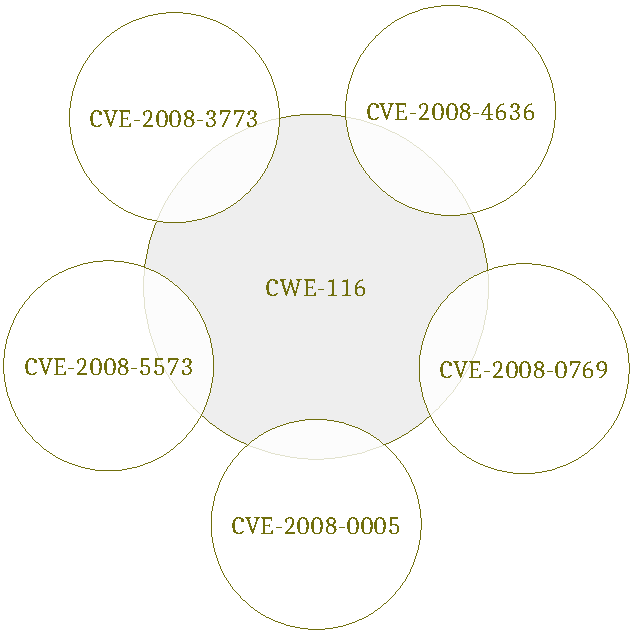
\includegraphics[width=.7\textwidth]{rcc5_CWE-116.pdf}
		\caption{Representation with RCC3}
		\label{fig:rcc5_CWE-116}
	\end{subfigure}\begin{subfigure}[b]{.5\textwidth}
		\centering
		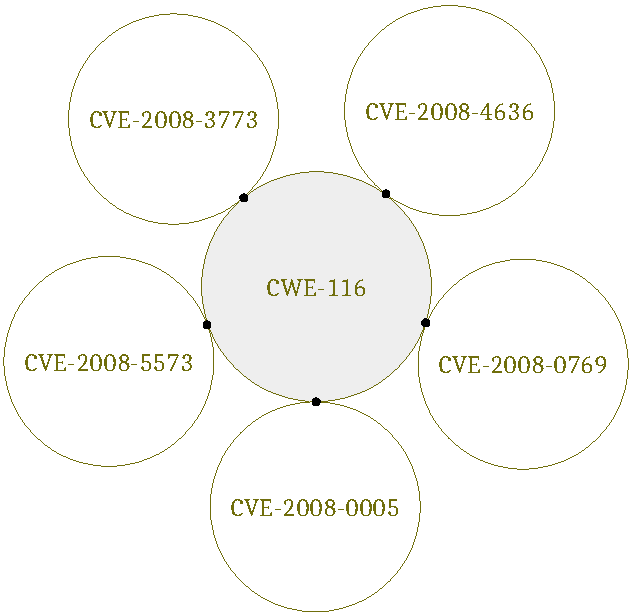
\includegraphics[width=.7\textwidth]{rcc8_CWE-116.pdf}
		\caption{Representation with RCC8}
		\label{fig:rcc8_CWE-116}
	\end{subfigure}
	\begin{subfigure}[b]{\textwidth}
		\centering
		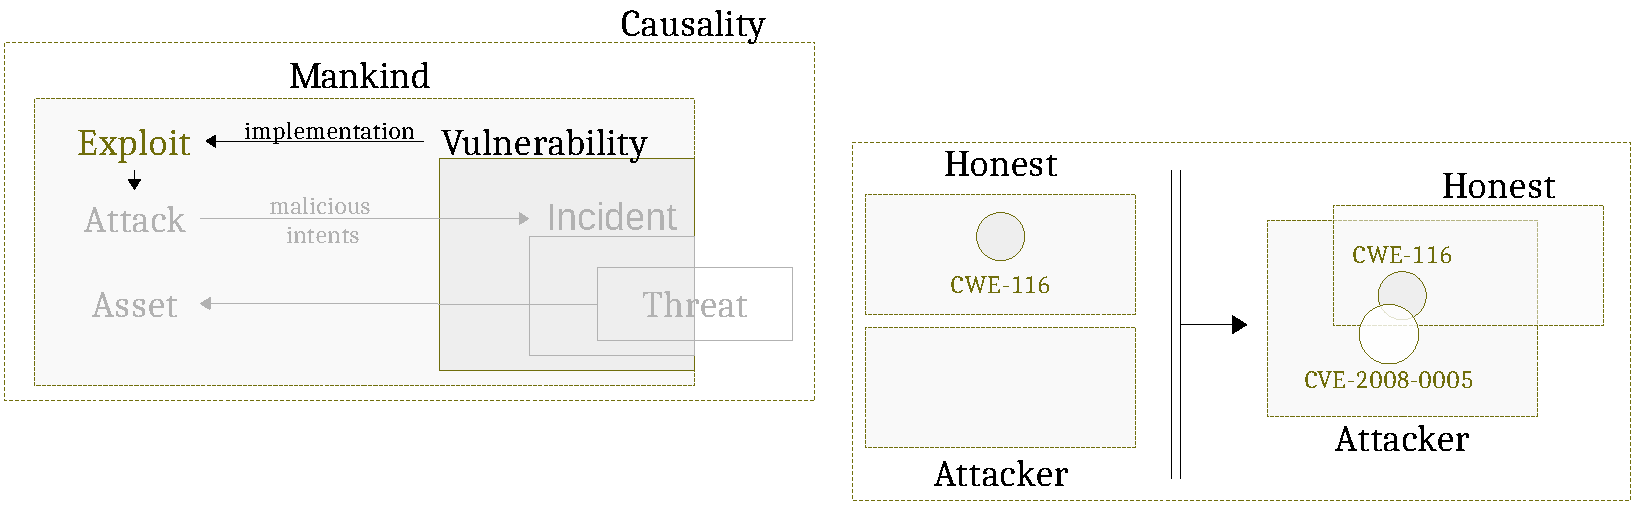
\includegraphics[width=\textwidth]{KML_CWE-116.pdf}
		\caption{Representation in K-Modal Logic}
		\label{fig:KML_CWE-116}
	\end{subfigure}
	\caption{Relations between CWE-116 and correlated CVEs}
\end{figure}
Definition~\ref{def:weakness} states that CWE-116 is a weakness iff there exists a world in
K Modal Logic, representing the system in which this weakness exists, 
such that the natural evolution of this system (i.e. formalized by the causality principle) 
make it possible to reach another state of the system (i.e. another, accessible world)
where there exist a vulnerability that can be implemented from CWE-116 (and this relation 
is not DR). The CWE website proposes the connection between CWE-116 and, for example, 
CVE-2008-5573; a vulnerability of the login sub-system 
of the Poll Pro v2.0\autocite{pollpro} system.
The formal relation between the two is given as a link (i.e. URI) between the CWE and
the CVE, the description of the relation is not defined but it is supposed to be
inferred from the descriptions of the CWE-CVE. 
We can formally represent this link as the ONE connection in RCC3, depicted in 
Figure~\ref{fig:rcc5_CWE-116}, or EC connection in RCC8 (Figure~\ref{fig:rcc8_CWE-116}).

\fixnote{mr}{shouldn't we consider the agent who introduces the weakness as dishonest? don't we say this in part 1?}
\end{example}

It is interesting to note that the CWE-CVE relation expresses the correlation
between weaknesses and vulnerabilities in the most simple form, such that we
can formalize all the relation as ONE in RCC3 or EC in RCC8.  To express a more
complex relation between the two we shall analyze the definition of CWE-116.
This is related to the Weakness-Vulnerability-Incident process (i.e. to the
details on the implementation/realization in Figure~\ref{fig:safety-security})
that we analyze in the next section, Section~\ref{sec:incidentaccident}.

\begin{definition}{\bf Region: Vulnerability and Defect --}\label{def:vulnerability-defect}
A region $\region\subseteq\agent$ of an agent $\agent\in\agentuniverse$ is
	called \emph{Vulnerability} if the agent $\agent$ is referred to as Mankind, 
	\emph{Defect} if the agent is referred to as Nature.
\end{definition}

\subsection{Process: Incidents and Accidents}\label{sec:incidentaccident}
In our informal definition depicted in Figure~\ref{fig:safety-security}, an
Incident is generated through a process caused by a Vulnerability (which,
in turn, is caused by a Weakness). Symmetrically, Nature has a process from Defect
to Accidents. We start by analyzing the process generated by Mankind, which is
divided into the following phases (as shown in Figure~\ref{fig:cwe-nvd-capec}):
\begin{enumerate}
	\item An agent (Mankind or Nature) defines a system, e.g. by following an engineering process for creating a new system, or for redesigning or improving an existing system (e.g. a component or a collection of components) 
	\item The dogmatic definition of a system contains a Weakness (i.e. the agent, Mankind or Nature, introduces an unintended behavior), for example as an un-intended behavior or as an architectural fallacy. The Weakness can be applied to the abstract definition of the system.
	\item The Weakness can be defined as a malicious process for a system, called Vulnerability (or Defect for Nature)
	\item The process expressed by the Vulnerability can be made operational for a specific implementation of the system (i.e. implemented by Mankind or realized by Nature) 
\end{enumerate}
Those additional details are depicted in Figure~\ref{fig:safety-security_2}, an update
of Figure~\ref{fig:safety-security}.

\begin{figure}[t]
	\centering
	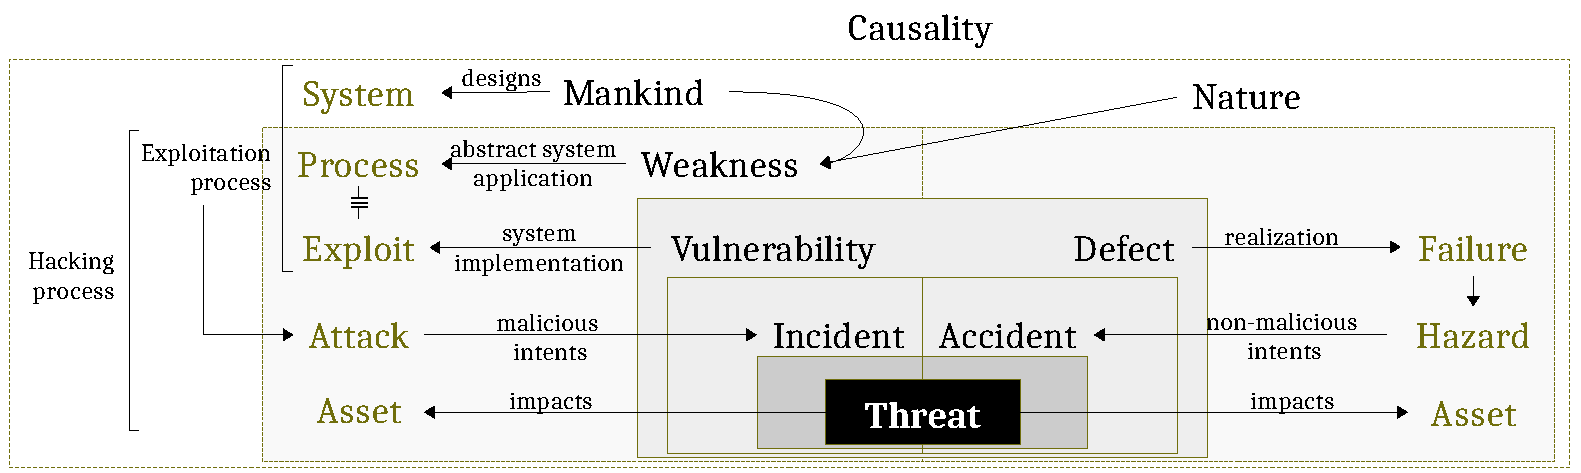
\includegraphics[width=\textwidth]{safety-security_2.pdf}
	\caption{Updated overview security and safety keywords, where Process
	has to be intended as ``Abstract Exploitation Process''}
	\label{fig:safety-security_2}
\end{figure}

\begin{definition}{\bf Exploitation Process --} An \emph{Exploit} is an \emph{implementation} of
a Vulnerability, where a Vulnerability describes how to transform a
Weakness into an abstract malicious process, which can be applied\footnote{Meaning that the
malicious process, i.e.  any structured procedure such as a protocol, can be
somehow made operational, e.g. implemented} to one or many systems. So, the act
of an agent (Mankind) of ``exploiting a Vulnerability'' is the process of
making the Vulnerability operational, by implementing the Vulnerability w.r.t.
a specific target system.  Whenever the agent is Nature, the implementation is
more broadly considered a realization\footnote{``The state of being
realized''\autocite{Merriam2020realization}}. 
\end{definition}

\begin{figure}[t]
	\centering
	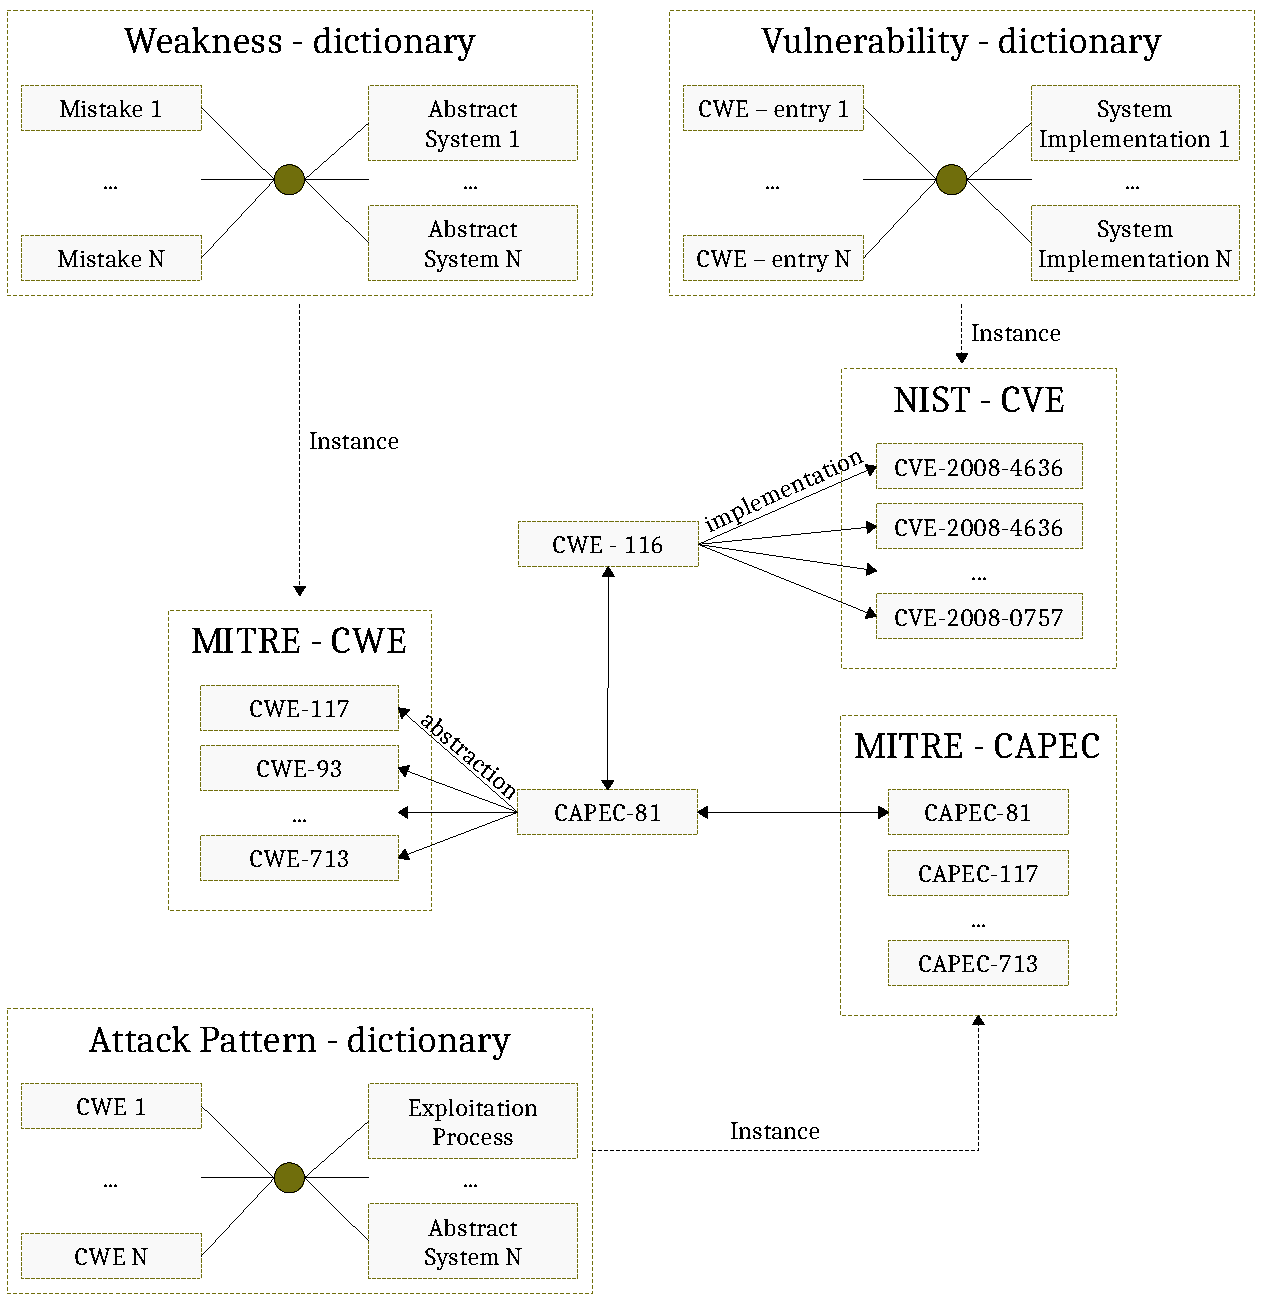
\includegraphics[width=\textwidth]{cwe-nvd-capec.pdf}
	\caption{Cybersecurity online dictionaries and connections}
	\label{fig:cwe-nvd-capec}
\end{figure}

The Common Attack Pattern Enumeration and
Classification\autocite{MITRE2020CAPEC} (CAPEC) online service provides a
``community resource'' which aims at ``identifying and understanding attacks''.
The MITRE writes on the CAPEC homepage that ``Understanding how the adversary
operates is essential to effective cyber security. CAPEC helps by providing a
comprehensive dictionary of known patterns of attack employed by adversaries to
exploit known weaknesses in cyber-enabled capabilities. It can be used by
analysts, developers, testers, and educators to advance community understanding
and enhance defenses.''. We can extrapolate two major concepts: 
\begin{itemize}
	\item While understanding the exploitation process is the aim of the
		CWE and CVE initiatives, understanding the hacking process is
		the aim of the CAPEC initiative.
	\item CAPEC provides a \emph{dictionary} of \emph{known} attack patterns.
		As stated in details in Section~\ref{sec:problem}, this dictionary contains
		empirical evidences and should not be used to induce a cybersecurity 
		theory; but it can be used to validate a theory.
\end{itemize}

\begin{example}
The CWE-116 doesn't just relate the Weakness to a number of Vulnerability in
	the CVE but also relates the Weakness to a number ($4$ for the CWE-116)
	of abstract attack path in the CAPEC:
	\begin{itemize}
		\item CAPEC-104\autocite{CAPEC-104} Cross Zone Scripting
		\item CAPEC-73\autocite{CAPEC-73} User-Controlled Filename
		\item CAPEC-81\autocite{CAPEC-81} Web Logs Tampering
		\item CAPEC-85\autocite{CAPEC-85} AJAX Fingerprinting
	\end{itemize}

	Each CAPEC entry has a reference to one or many CWE, including CWE-116.
\end{example}

After the exploitation process, as depicted in Figure~\ref{fig:cwe-nvd-capec},
another process starts and transforms a Vulnerability in an Incident by
Attacking the system with a malicious Hack, as follows.
\begin{enumerate}
\setcounter{enumi}{4}
	\item An agent (Mankind\footnote{For the sake of readability we focus
		only on Mankind as an agent}) the exploitation process can be
		used to hack a system. We use the term hack (as hacking) to
		stress that nothing prevents this process from being honest,
		however, for the sake of simplicity, we focus on Attacks which
		are malicious by definition.
	\item An Attack is applied to a system with malicious intent by an
		agent
	\item The application of the attack results in an Incident which
		impacts, i.e. poses a Threat to, an Asset
\end{enumerate}

\begin{definition}{\bf Black-hat Hacking Process}\label{def:hackingprocess}
An \emph{Attack} is the act of making operational an \emph{Exploitation Process} 
	causing an Incident. 
\end{definition}

\begin{example}	CAPEC-81\autocite{CAPEC-81} Web Logs Tampering --
	\begin{itemize}
		\item Description: An attacker is able to cause a victim to
			load content into their web-browser that bypasses
			security zone controls and gain access to increased
			privileges to execute scripting code or other web
			objects such as unsigned ActiveX controls or applets.
			This is a privilege elevation attack targeted at
			zone-based web-browser security. In a zone-based model,
			pages belong to one of a set of zones corresponding to
			the level of privilege assigned to that page. Pages in
			an untrusted zone would have a lesser level of access
			to the system and/or be restricted in the types of
			executable content it was allowed to invoke. In a
			cross-zone scripting attack, a page that should be
			assigned to a less privileged zone is granted the
			privileges of a more trusted zone. This can be
			accomplished by exploiting bugs in the browser,
			exploiting incorrect configuration in the zone
			controls, through a cross-site scripting attack that
			causes the attackers' content to be treated as coming
			from a more trusted page, or by leveraging some piece
			of system functionality that is accessible from both
			the trusted and less trusted zone. This attack differs
			from "Restful Privilege Escalation" in that the latter
			correlates to the inadequate securing of RESTful access
			methods (such as HTTP DELETE) on the server, while
			cross-zone scripting attacks the concept of security
			zones as implemented by a browser. 
		\item Execution Flow: 
			\begin{enumerate}
				\item Explore: Find systems susceptible to the
					attack: Find systems that contain
					functionality that is accessed from
					both the internet zone and the local
					zone. There needs to be a way to supply
					input to that functionality from the
					internet zone and that original input
					needs to be used later on a page from a
					local zone. 
				\item Experiment: Find the insertion point for
					the payload: The attacker first needs
					to find some system functionality or
					possibly another weakness in the system
					(e.g. susceptibility to cross site
					scripting) that would provide the
					attacker with a mechanism to deliver
					the payload (i.e. the code to be
					executed) to the user. The location
					from which this code is executed in the
					user's browser needs to be within the
					local machine zone.
				\item Exploit: Craft and inject the payload:
					Develop the payload to be executed in
					the higher privileged zone in the
					user's browser. Inject the payload and
					attempt to lure the victim (if
					possible) into executing the
					functionality which unleashes the
					payload.
			\end{enumerate}
		\item Prerequisite: The target must be using a zone-aware browser. 
		\item Consequences: 
			\begin{itemize}
				\item Integrity: Modify Data
				\item Confidentiality: Read Data
				\item Confidentiality, Access Control, Authorization: Gain Privileges
				\item Confidentiality, Integrity, Availability: Execute Unauthorized Commands
			\end{itemize}
	\end{itemize}

\end{example}

The formalization of the Exploitation and Black-hat Hacking processes is the
formalization of two foundational cybersecurity concepts which lay the basis
for the definition (and formalization) of the cybersecurity theory in the next
Section (Section~\ref{sec:theory}). The formal definition of those
processes shall:
\begin{itemize}
	\item in Section~\ref{sec:theory}, formally define a system as a structure of agents, and
	\item in Section~\ref{sec:engineering}, correlate the formal definition of agents (i.e. the
		Definition~\ref{def:agent}) with the Causality principle (i.e.
		the formalization of the Kripke structure in
		Definition~\ref{def:modallogic}). 
\end{itemize}
